\subsubsection{数据接口、候选动作与资源约束}
问题一的每条冲突边都必须在调整后的完整重复事件上重新检查。按假设（2），对每份计划 \(i\) 构造候选动作集合 \(\mathcal A_i\)，其中包含保留、频率平移、时间平移和撤销。频率平移量满足 \(\lvert\Delta f\rvert\le 10\)，时间平移量满足 \(\lvert\Delta t\rvert\le 5\)，并且一份计划不能同时改变频率和时间。所有候选动作均保持原计划的单次时长、间隔时长和使用次数不变；按假设（3）在进入模型前删除越过资源域的候选。

令 \(x_{ia}\in\{0,1\}\) 表示计划 \(i\) 是否选择动作 \(a\)，令 \(\mathcal K_{ia}\) 表示该候选动作展开后占用的离散时频资源格集合。每份计划恰选择一个候选动作：
\begin{equation}
\sum_{a\in\mathcal A_i}x_{ia}=1,\qquad i\in\mathcal I.
\label{eq:q2-one-action}
\end{equation}
对任一资源格 \(c\)，最多允许一个候选动作占用：
\begin{equation}
\sum_{(i,a):\,c\in\mathcal K_{ia}}x_{ia}\le 1.
\label{eq:q2-cell-clique}
\end{equation}
该资源格约束等价于对候选动作逐对加入冲突约束，但能够把 270\,626 条候选成对冲突边压缩为 52\,939 条资源格团约束。基准场景共形成 4\,582 个合法候选动作。

\subsubsection{条件字典序目标}
题面只给出“尽可能少撤销、少调整并优先保护高等级装备”的定性要求，直接设置任意数值权重会使结果依赖人为尺度。因此采用条件字典序
\begin{equation}
(R,\ R_A,\ R_B,\ M,\ M_A,\ M_B,\ S_{10}),
\label{eq:q2-lexicographic}
\end{equation}
逐层求解并在每层获得上下界一致或阈值不可行证据后固定该层。这里 \(R\) 为总撤销数，\(M\) 为被调整计划数，下标 \(A,B\) 表示相应类别。末级平移量定义为
\begin{equation}
S_{10}=\sum_i\left(\lvert\Delta f_i\rvert+2\lvert\Delta t_i\rvert\right)
=10\sum_i\left(\frac{\lvert\Delta f_i\rvert}{10}+
\frac{\lvert\Delta t_i\rvert}{5}\right).
\label{eq:q2-shift-score}
\end{equation}
式 \eqref{eq:q2-shift-score} 用于固定前六层后的末级并列破除；其相邻阈值不可行性也需要单独证明。

\subsubsection{模型求解与已闭合前缀}
主模型使用 CP-SAT 求解资源格约束\cite{ortools}，关键次级目标再用独立 CNF 阈值模型和 CaDiCaL\cite{cadical} 检查“更优一档是否不可行”。得到的前缀证据如下。

\begin{table}[H]
\centering
\caption{问题二条件字典序前缀的上下界证据}
\label{tab:q2-proof}
\begin{tabular}{lrrl}
\toprule
目标层 & 下界 & 上界 & 结论 \\
\midrule
总撤销 \(R\) & 6 & 6 & 已证明最优 \\
A 类撤销 \(R_A\mid R=6\) & 0 & 0 & 已证明条件最优 \\
B 类撤销 \(R_B\mid R=6,R_A=0\) & 4 & 4 & 已证明条件最优 \\
总调整 \(M\mid\text{前缀固定}\) & 126 & 126 & 已证明条件最优 \\
A 类调整 \(M_A\mid\text{前缀固定}\) & 16 & 16 & 已证明条件最优 \\
B 类调整 \(M_B\mid\text{前缀固定}\) & 34 & 34 & 已证明条件最优 \\
末级平移 \(S_{10}\mid\text{前六层固定}\) & 775 & 775 & 已证明条件最优 \\
\bottomrule
\end{tabular}
\end{table}

因此，当前已证明的完整条件字典序结果为
\[
(R,R_A,R_B,M,M_A,M_B,S_{10})=(6,0,4,126,16,34,775).
\]
其中 \(R\) 的上下界来自 CP-SAT 的最优证书；B 类撤销数、三层调整数和末级平移量的下界由独立 CNF 阈值不可行证明给出。末级证书在完整 4\,582 个候选动作全集上检验 \(S_{10}\le774\) 不可行。

表 \ref{tab:q2-proof} 已经完整给出每一层的上下界和证明状态，因此不再另设证明阶梯图，避免用图形重复同一组离散证据。

\subsubsection{六撤销方案与结果}
在上述前缀下得到的正式方案按类别统计如下。

\begin{table}[H]
\centering
\caption{问题二正式方案的类别构成}
\label{tab:q2-solution}
\begin{tabular}{lrrr}
\toprule
类别 & 保留 & 调整 & 撤销 \\
\midrule
A & 4 & 16 & 0 \\
B & 2 & 34 & 4 \\
C & 12 & 76 & 2 \\
\midrule
合计 & 18 & 126 & 6 \\
\bottomrule
\end{tabular}
\end{table}

撤销计划为 B009、B018、B024、B028、C027 和 C054。方案保留 144 个活动计划，占用 15\,816 个不同资源格；频移绝对值总和为 595，时移绝对值总和为 90，因而当前方案的 \(S_{10}=775\)。

图 \ref{fig:q2-composition} 展示同一动作表的类别构成。A 类没有撤销，B 类承担 4 次撤销，C 类保留 12 条、调整 76 条并撤销 2 条；这张图只用于呈现动作组成，不替代前缀证明。

\begin{figure}[htbp]
  \centering
  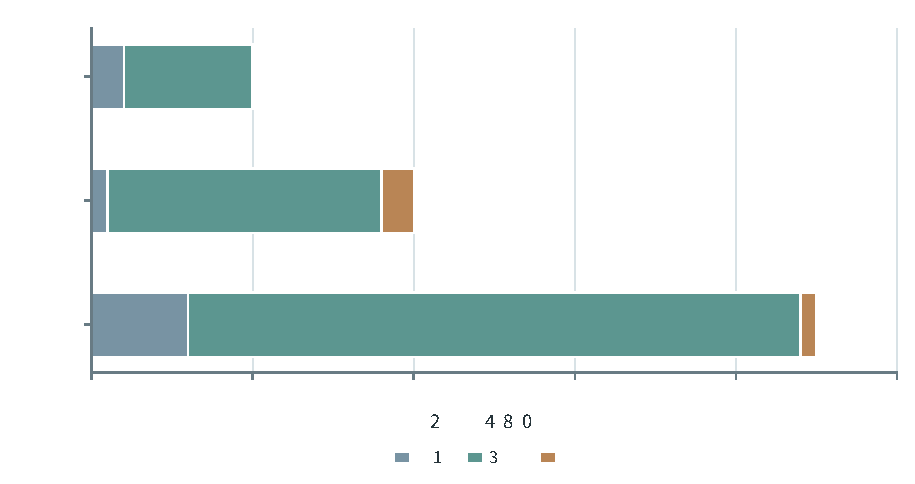
\includegraphics[width=0.88\textwidth]{figures/fig4_q2_composition.pdf}
  \caption{问题二正式方案的类别构成}
  \label{fig:q2-composition}
\end{figure}

\subsubsection{独立可行性检验}
验证程序从动作表重新读取原始附件，并分别用连续半开区间和离散资源格复核全部重复事件。两种方法均得到零冲突、零越界和零重复占用，最大单元占用数为 1。结果工作簿只填写发生变化的参数列，132 条动作行通过工作簿格式检查。该六撤销方案作为问题三的冻结输入，不由问题三的新增容量反向修改。

\subsubsection{最优性边界}
末级平移量也已闭合：在固定 \((R,R_A,R_B,M,M_A,M_B)=(6,0,4,126,16,34)\) 后，完整候选全集上的独立 CNF 模型返回 \(S_{10}\le774\) 为 \texttt{UNSAT}；正式方案给出 \(S_{10}=775\)，故末级上下界一致。该结论只针对本文明确的有限动作集合、半开区间和 \(H=643\) 资源域。

\subsubsection{问题二小结}
问题二把 Q1 的冲突边转化为候选动作之间的资源格互斥关系，得到总撤销数为 6 的已验证方案，并对高层目标、类别保护目标和末级平移量均给出上下界证据。
